\chapter{Aufgabe 3}

\section{a)}

\textit{Entwurf des Dateisystems einschließlich einer Beschreibung der in den Dateien
gespeicherten Daten.}\\

\noindent
Es folgt eine grobe Beschreibung der Datei-Struktur der Anwendung, die in Abbildung~\ref{fig:struktur} und in Tabelle~\ref{tab:struktur} zusätzlich gelistet ist.
Die Nummerierung der Dateien (Subskripte) dient hierbei der Veranschaulichung :

\begin{itemize}
    \itemsep0.5em
    \item \textbf{DF - Dedicated Files}
    \begin{itemize}
        \item \textit{MF}: Wurzelverzeichnis der Chipkarte
        \item \textit{DF$_1$}: Wurzelverzeichnis der SSO-Cipkartenanwendung, beinhaltet Schlüssel, PIN, Anwendungsdaten
    \end{itemize}
    \item \textbf{EF - Elementary Files}
    \begin{itemize}
    \item \textit{DF$_1$.EF$_1$} (\textbf{Cyclic}): Da eine PIN-Eingabe erfolgt, muss die Anwendung auf der Chipkarte die Anzahl der Fehlversuche
    für eine mögliche Sperrung der Karte protokollieren.
    Hierfür wird der Befehl \texttt{INCREASE} / \texttt{DECREASE} genutzt,
    der nach ISO/IEC 7816 diesem Dateityp zur Verfügung steht (vgl.~\cite[45]{ITS5})
    \item \textit{DF$_1$.EF$_2$} (\textbf{Linear Fixed}): Dateityp fixer Länge zur Speicherung der PIN.
    Sicherheitsattribute (\textit{EF$_2$.ARR}): Access-Mode \texttt{READ-ONLY}.
    \item  \textit{DF$_1$.EF$_3$} (\textbf{Linear Fixed}): Dateityp fixer Länge zur Speicherung des Schlüssels.
    Sicherheitsattribute (\textit{EF$_3$.ARR}): Access-Mode \texttt{READ-ONLY}, PIN-verifikation erforderlich
    \end{itemize}
\end{itemize}

\begin{table}[h]
    \setlength{\tabcolsep}{0.5em}
    \def\arraystretch{1.5}
    \centering
    \begin{tabular}{|l|c|l|p{7cm}|}
        \hline
        \textbf{Datei} & \textbf{FID} & \textbf{Struktur} & \textbf{Beschreibung} \\
        \hline
        MF & $3F00$ & Top-Level Dedicated File & Wurzelverzeichnis der Chipkarte \\
        \hline
        DF$_1$ & -- & Dedicated File & Verzeichnis der SSO-Anwendung \\
        \hline
        DF$_1$.EF$_1$ & $0001$ & Cyclic & Protokollierung von Fehlversuchen bei PIN-Eingabe (Sperrzähler), nutzbar mit \texttt{INCREASE}/\texttt{DECREASE} \\
        \hline
        DF$_1$.EF$_2$ & $0002$ & Linear Fixed & Speicherung der PIN \\
        \hline
        DF$_1$.EF$_3$ & $0003$ & Linear Fixed & Speicherung des privaten Schlüssels für SSO-Anmeldung \\
        \hline
        DF$_1$.EF$_2$.ARR & -- & -- & Zugriffsschutzdefinition für DF$_2$.EF$_1$, \texttt{READ-ONLY} \\
        \hline
        DF$_1$.EF$_3$.ARR & -- & -- & Zugriffsschutzdefinition für DF$_2$.EF$_2$, \texttt{READ} nach PIN-Verifikation, nicht exportierbar \\
        \hline
    \end{tabular}
\caption{Übersicht über die Dateistruktur der SSO-Chipkartenanwendung nach ISO/IEC 7816. (Quelle: Struktur und Notation in Anlehnung an~\cite[\textbf{Tabelle 15.11}, 897]{RE02})}
\label{tab:struktur}
\end{table}


\begin{figure}
    \centering
    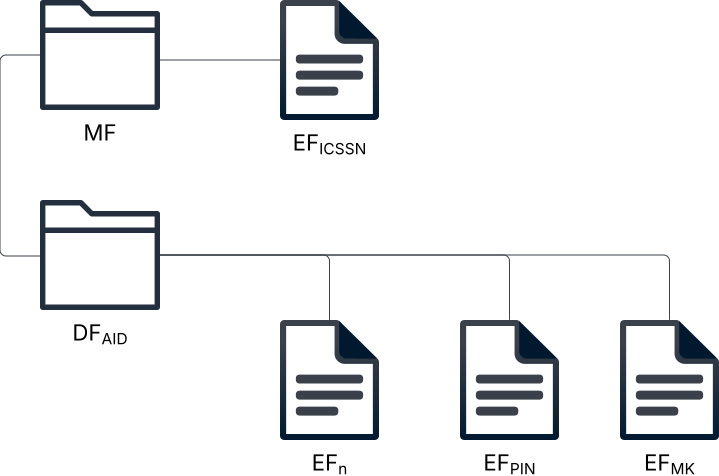
\includegraphics[scale=0.4]{aufgabe 3/img/struktur.svg}
    \caption{Skizze der Dateistruktur als Lösungsvorschlag für die in Aufgabe 3 beschriebene Chipkartenanwenung. (Quelle: eigene)}
    \label{fig:struktur}
\end{figure}